\documentclass[
  a4paper,
  11pt,
]{article}

\usepackage[utf8]{inputenc}
\usepackage[cm, headings]{fullpage}
\usepackage[ngerman]{babel}
\usepackage{amsmath}
\usepackage{amssymb}
\renewcommand{\O}{\mathcal{O}}

\usepackage{color}
\definecolor{mygray}{rgb}{0.5,0.5,0.5}
\usepackage{listings}
\usepackage{tikz}
\usepackage{pgfplots}
\usepackage{booktabs}

% Für Zeilenumbrüche ohne Indentations
\setlength{\parindent}{0pt}

\lstset{%
  basicstyle=\ttfamily,
  keywordstyle=\color{blue},
  commentstyle=\color{mygray},
  language=C,
  showstringspaces=false,
}


% Grafikpaket laden
\usepackage{graphicx}
\usepackage{float}

% coole Kopf- und Fußzeilen:
\usepackage{fancyhdr}
% Seitenstil ist natürlich fancy:
\pagestyle{fancy}
% alle Felder löschen:
\fancyhf{}

\fancyhead[L]{%
  Seminar: Public-Key-Kryptographie
}
\fancyhead[R]{%
}
%\fancyfoot[L]{}
\fancyfoot[C]{\thepage}

\newcommand{\N}{\mathbb{N}}
\newcommand{\Z}{\mathbb{Z}}
\newcommand{\ggT}{\text{ggT}}

\title{}

\author{}

\begin{document}

Diskreter Logarithmus:
\\\\
source: Übersetzung aus HAC97 Seite 103
\\\\
Definition:
\\\\
The discrete logarithm problem (DLP) is the following:

%$Z_p^* = \{ 0 ,\ldots , p - 1 \} , {a,b\in \{0,\ldots ,p-1\},\,}$\\
%$g^{{ab}}$			%g hoch a*b
%$a\equiv b\mod m$	%kongruenz

$Z_p^* = \{ 0 ,\ldots , p - 1 \}$

given a prime p, a generator ${a\in Z_p^*}$, and an element ${b\in Z_p^*}$,
find the integer x, $0\leq x\leq p-2$, such that
a hoch x kongruent b (mod p)
\\\\
Das Diskrete-Logarithmus-Problem:
Für eine Primzahl p, eine multiplikative Gruppe $Z_p^* = \{ 0 ,\ldots , p - 1 \}$, einen Generator ${a\in Z_p^*}$ und ein ${b\in Z_p^*}$,
finde ${x\in N}$, $0\leq x\leq p-2$ (oder auch $1\leq x\le p-1$, zyklische Gruppe),
so dass a hoch %$x\equiv b\mod p$.

\subsection*{Diffie-Hellman-Merkle Schluesselaustausch (DHKE)}
\label{sub:Diffie-Hellman-Merkle Schluesselaustausch (DHKE)}

	Alice\\
	1.\\
	Wähle:	Primzahl $p$\\
	Finde:	Erzeuger $g$:\\
			$g^n\text{ }mod\text{ }p \rightarrow \{ 0 ,\ldots , p - 1 \}$\\
	Wähle:	Geheimen Schlüssel: $a\in \{ 1 ,\ldots , p - 1 \}$\\
	Berechne:	Öffentlichen Schlüssel: $A=g^a\text{ }mod\text{ }p$\\
	Sende: (p, g, A) an Bob\\\\

	Bob\\
	2.\\
	Wähle:	Geheimen Schlüssel: $b\in \{ 1 ,\ldots , p - 1 \}$\\
	Berechne:	Öffentlichen Schlüssel: $B=g^b\text{ }mod\text{ }p$\\
	Berechne:	Geheimen gemeinsamen Schlüssel: $K=A^b\text{ }mod\text{ }p$\\
	Sende: (B) an Alice\\\\
	
	Alice\\
	3.\\
	Berechne:	Geheimen gemeinsamen Schlüssel: $K=B^a\text{ }mod\text{ }p$\\

\begin{figure}[H]
	\centering
	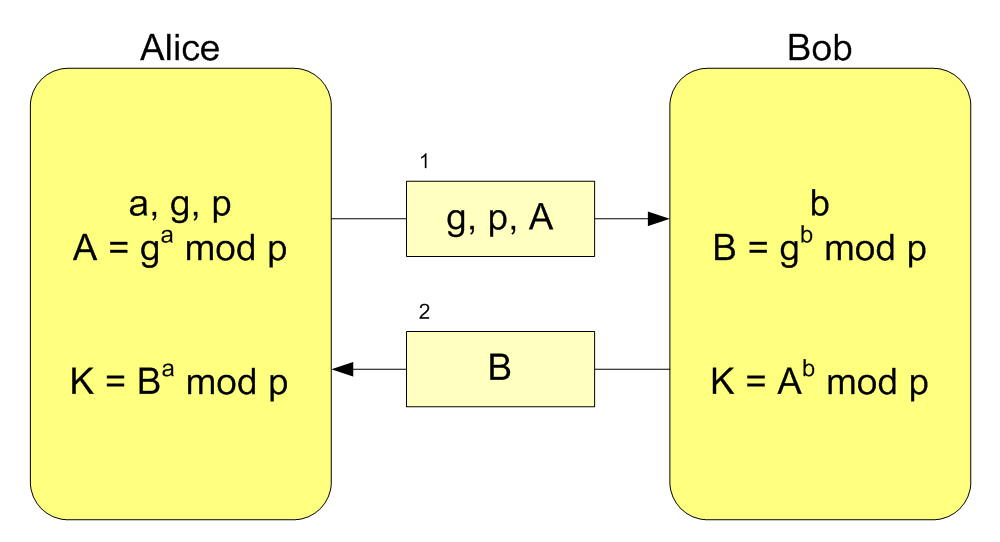
\includegraphics[width=\textwidth]{Diffie-Hellman-Schluesselaustausch2.png}
	\caption{Diffie-Hellman-Merkle Schluesselaustausch}
	\label{img:grafik-dummy}
\end{figure}

\subsection*{DHKE: Beweis, Korrektheit}
\label{sub:DHKE: Beweis, Korrektheit}

\begin{center}
\begin{tabular}{rcl}
	$K1$	&	$=$ &	$B^a\text{ }mod\text{ }p$\\
			&	$=$	&	$(g^b)^a\text{ }mod\text{ }p$\\
			&	$=$	&	$g^{ba}\text{ }mod\text{ }p$\\
			&	$=$	&	$g^{ab}\text{ }mod\text{ }p$\\
			&	$=$	&	$(g^a)^b\text{ }mod\text{ }p$\\
			&	$=$	&	$A^b\text{ }mod\text{ }p$\\
			&	$=$	&	$K2$\\
\end{tabular}
\end{center}

\subsection*{Verschluesselung}
\label{sub:Verschluesselung}

Grundsätzlich wie DHKE, wobei Bob (Sender) zusätzlich zu seinem öffentlichen Schlüssel die chiffrierte Nachricht mitsendet. Dabei kann der Empfänger (Alice)
seinen öffentlichen Schlüssel bereits LANGE VOR der Übertragung der Nachricht bekanntgeben.\\\\

Sender (Bob)\\
Hat: öffentlichen Schlüssel des Empfängers (Alice): (p, g, A)\\
2.	zusätzlich:\\
	Nachricht: ${m\in \mathbb{N}^n}$ - Text der Länge $n$ auf Zahlen abbilden.\\
	Verschlüsselung:	$c_i=A^b\cdot m_i\mod p$\\
	Sendet:	(B, c)

Empfänger (Alice)\\
Hat: (p, g, A, a, B, c)\\
3.	zusätzlich:\\
	Entschlüsselung:	$m_i=B^{-a}\cdot c_i\mod p$\\
	$m_i=B^{(p-1)-a}\cdot c_i\mod p$
	
An dieser stelle sei darauf verwiesen, dass zusätzliche Maßnahmen getroffen werden müssen, da jeder Buchstabe auf die selbe Zahl verschlüsselt wird.
Z.B.: Mehrere Buchstaben zusammenfassen

\subsection*{Verschluesselung: Beweis, Korrektheit}
\label{sub:Verschluesselung: Beweis, Korrektheit}

%\subsubsection*{Theorie}
%\label{subsub:Theorie}
%
%$c=A^b\cdot m\mod p$\\
%$m=B^{-a}\cdot c\mod p$\\
%
%\subsubsection*{Beweis, Korrektheit}
%\label{subsub:Beweis, Korrektheit}

\begin{center}

\begin{tabular}{rl}
	Chiffre Text:	&	$c=A^b\cdot m\mod p$\\
	Message:		&	$m=B^{-a}\cdot c\mod p$\\
\end{tabular}

\ \\ \ \\

\begin{tabular}{rcl}
	$m$		&	$=$ &	$B^{-a}\cdot c\mod p$\\
			&	$=$	&	$(g^b)^{-a}\cdot c\mod p$\\
			&	$=$	&	$g^{b\cdot (-a)}\cdot c\mod p$\\			
			&	$=$	&	$g^{-ab}\cdot c\mod p$\\
			&	$=$	&	$g^{-ab}\cdot A^b\cdot m\mod p$\\
			&	$=$	&	$g^{-ab}\cdot (g^a)^b\cdot m\mod p$\\
			&	$=$	&	$g^{-ab}\cdot g^{ab}\cdot m\mod p$\\
			&	$=$	&	$g^{-ab+ab}\cdot m\mod p$\\
			&	$=$	&	$m$\\
\end{tabular}
\end{center}

\subsection*{Komplexitaet}
\label{sub:Komplexitaet}

Diskreter Logarithmus: $DL(y, g, p) = x$ für $g^x=y\mod p$\\
- kein direktes Verfahren: Brute Force über $\{1, \ldots, x\}\in \mathcal O(x)$\\
- Länge von x in bit: n $\rightarrow \mathcal O(2^n)$\\\\

Angenommen:\\
- Ein Prozessor mit 10 GHz ($= 10^{10}Hz$),\\
kann mit jedem Schritt eine modulare Potenz berechnen: $exp(x,g,p)=g^x\mod p$\\
- Anzahl Prozessoren: $k=10^{10} \rightarrow 10^{20}$ modulare Potenzen pro Sekunde $\approx 2^{67} 1/s$\\
- Die Zeit zur Berechnung aller modularen Potenzen: $t=2^n/(2^{67}\cdot s^{-1})$\\\\

Man kann $x=2^n$ so setzen, dass $t>t_{alter des Universum}$:\\
$t_{alter des Universum}=14\cdot 10^9y=14\cdot 10^9\cdot 365\cdot 24\cdot 60\cdot 60\cdot s\approx 2^{59}\cdot s$\\
$59=n-67\rightarrow n=59+67\rightarrow n=126$





\end{document}
